\documentclass[tikz,border=5mm]{standalone}
\usepackage[T1]{fontenc}
\usepackage{lmodern}
\usepackage{amsmath,amssymb}
\usepackage{xcolor}
\usepackage{tikz}
\usetikzlibrary{arrows.meta,positioning,calc,fit,backgrounds,decorations.pathreplacing,shapes.geometric}
\definecolor{leafgreen}{HTML}{54A24B}
\definecolor{errorred}{HTML}{E45756}
\definecolor{okblue}{HTML}{4C78A8}
\tikzset{
  sknode/.style = {rectangle, draw=black!60, fill=white, rounded corners=2pt,
                   minimum width=1.5cm, minimum height=0.6cm, inner sep=3pt,
                   font=\sffamily\fontsize{8}{9.5}\selectfont, align=center},
  valnode/.style = {font=\sffamily\bfseries\fontsize{9}{10.5}\selectfont},
  opnode/.style = {rectangle, draw=black!35, fill=black!3, rounded corners=2pt,
                   minimum width=0.9cm, minimum height=0.35cm, inner sep=2pt,
                   font=\sffamily\fontsize{6.5}{8}\selectfont, align=center},
  erranno/.style = {font=\sffamily\bfseries\fontsize{7.5}{9}\selectfont, text=errorred},
  okanno/.style = {font=\sffamily\bfseries\fontsize{7.5}{9}\selectfont, text=okblue},
}
\begin{document}
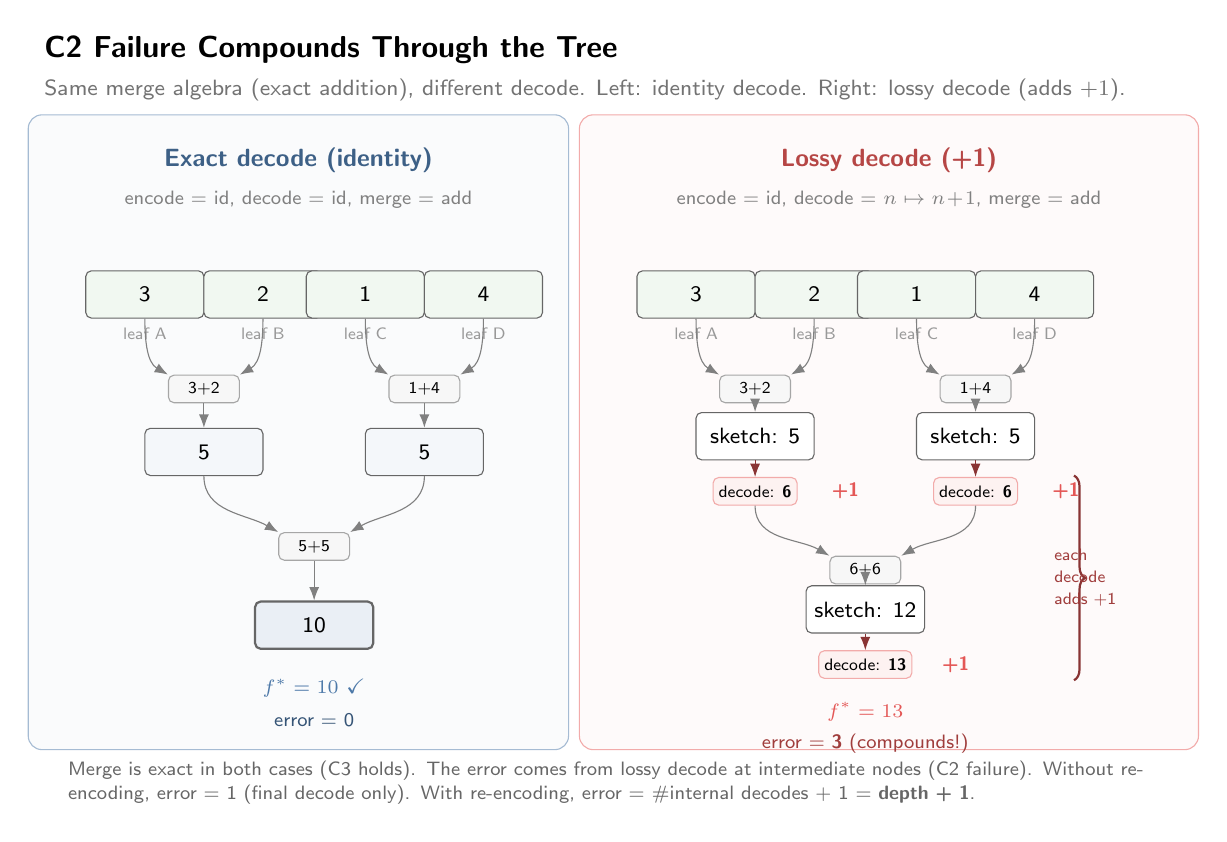
\begin{tikzpicture}[x=1cm,y=1cm,font=\sffamily,>=Latex]

  % Title
  \node[anchor=west, font=\sffamily\bfseries\fontsize{11}{13}\selectfont] at (0, 8.6)
    {C2 Failure Compounds Through the Tree};
  \node[anchor=west, font=\sffamily\fontsize{8}{9.5}\selectfont, text=black!55] at (0, 8.1)
    {Same merge algebra (exact addition), different decode.
     Left: identity decode. Right: lossy decode (adds $+1$).};

  % === LEFT PANEL: Exact decode ===

  \begin{scope}[on background layer]
    \node[draw=okblue!50, fill=okblue!3, rounded corners=5pt, inner sep=8pt,
          fit={(0.2,0.0) (6.5,7.5)}] {};
  \end{scope}

  \node[font=\sffamily\bfseries\fontsize{9.5}{11}\selectfont, text=okblue!80!black] at (3.35, 7.2)
    {Exact decode (identity)};
  \node[font=\sffamily\fontsize{7.5}{9}\selectfont, text=black!50] at (3.35, 6.7)
    {encode = id, decode = id, merge = add};

  % Leaves
  \node[sknode, fill=leafgreen!8] (eA) at (1.4, 5.5) {\valnode 3};
  \node[sknode, fill=leafgreen!8] (eB) at (2.9, 5.5) {\valnode 2};
  \node[sknode, fill=leafgreen!8] (eC) at (4.2, 5.5) {\valnode 1};
  \node[sknode, fill=leafgreen!8] (eD) at (5.7, 5.5) {\valnode 4};

  \node[font=\sffamily\fontsize{6.5}{8}\selectfont, text=black!40] at (1.4, 5.0) {leaf A};
  \node[font=\sffamily\fontsize{6.5}{8}\selectfont, text=black!40] at (2.9, 5.0) {leaf B};
  \node[font=\sffamily\fontsize{6.5}{8}\selectfont, text=black!40] at (4.2, 5.0) {leaf C};
  \node[font=\sffamily\fontsize{6.5}{8}\selectfont, text=black!40] at (5.7, 5.0) {leaf D};

  % Merge AB
  \node[opnode] (eOpAB) at (2.15, 4.3) {3+2};
  \node[sknode, fill=okblue!6] (eAB) at (2.15, 3.5) {\valnode 5};
  \draw[->, black!50] (eA.south) to[out=-90,in=150] (eOpAB.north west);
  \draw[->, black!50] (eB.south) to[out=-90,in=30] (eOpAB.north east);
  \draw[->, black!50] (eOpAB) -- (eAB);

  % Merge CD
  \node[opnode] (eOpCD) at (4.95, 4.3) {1+4};
  \node[sknode, fill=okblue!6] (eCD) at (4.95, 3.5) {\valnode 5};
  \draw[->, black!50] (eC.south) to[out=-90,in=150] (eOpCD.north west);
  \draw[->, black!50] (eD.south) to[out=-90,in=30] (eOpCD.north east);
  \draw[->, black!50] (eOpCD) -- (eCD);

  % Root merge
  \node[opnode] (eOpR) at (3.55, 2.3) {5+5};
  \node[sknode, fill=okblue!12, line width=0.8pt] (eRoot) at (3.55, 1.3) {\valnode 10};
  \draw[->, black!50] (eAB.south) to[out=-90,in=150] (eOpR.north west);
  \draw[->, black!50] (eCD.south) to[out=-90,in=30] (eOpR.north east);
  \draw[->, black!50] (eOpR) -- (eRoot);

  % Result
  \node[okanno] at (3.55, 0.5) {$f^\ast = 10$ \checkmark};
  \node[font=\sffamily\fontsize{7}{8.5}\selectfont, text=okblue!70!black] at (3.55, 0.1)
    {error = 0};

  % === RIGHT PANEL: Lossy decode ===

  \begin{scope}[on background layer]
    \node[draw=errorred!50, fill=errorred!3, rounded corners=5pt, inner sep=8pt,
          fit={(7.2,0.0) (14.5,7.5)}] {};
  \end{scope}

  \node[font=\sffamily\bfseries\fontsize{9.5}{11}\selectfont, text=errorred!80!black] at (10.85, 7.2)
    {Lossy decode (+1)};
  \node[font=\sffamily\fontsize{7.5}{9}\selectfont, text=black!50] at (10.85, 6.7)
    {encode = id, decode = $n \mapsto n\!+\!1$, merge = add};

  % Leaves
  \node[sknode, fill=leafgreen!8] (lA) at (8.4, 5.5) {\valnode 3};
  \node[sknode, fill=leafgreen!8] (lB) at (9.9, 5.5) {\valnode 2};
  \node[sknode, fill=leafgreen!8] (lC) at (11.2, 5.5) {\valnode 1};
  \node[sknode, fill=leafgreen!8] (lD) at (12.7, 5.5) {\valnode 4};

  \node[font=\sffamily\fontsize{6.5}{8}\selectfont, text=black!40] at (8.4, 5.0) {leaf A};
  \node[font=\sffamily\fontsize{6.5}{8}\selectfont, text=black!40] at (9.9, 5.0) {leaf B};
  \node[font=\sffamily\fontsize{6.5}{8}\selectfont, text=black!40] at (11.2, 5.0) {leaf C};
  \node[font=\sffamily\fontsize{6.5}{8}\selectfont, text=black!40] at (12.7, 5.0) {leaf D};

  % Merge AB (sketch level: exact)
  \node[opnode] (lOpAB) at (9.15, 4.3) {3+2};
  \node[sknode, fill=white] (lABsketch) at (9.15, 3.7) {\footnotesize sketch: 5};
  \draw[->, black!50] (lA.south) to[out=-90,in=150] (lOpAB.north west);
  \draw[->, black!50] (lB.south) to[out=-90,in=30] (lOpAB.north east);
  \draw[->, black!50] (lOpAB) -- (lABsketch);

  % Decode + re-encode (C2 violation)
  \node[opnode, fill=errorred!8, draw=errorred!50] (lDecAB) at (9.15, 3.0) {decode: \textbf{6}};
  \draw[->, errorred!60!black] (lABsketch) -- (lDecAB);
  \node[erranno, anchor=west] at (10.0, 3.0) {+1};

  % Merge CD
  \node[opnode] (lOpCD) at (11.95, 4.3) {1+4};
  \node[sknode, fill=white] (lCDsketch) at (11.95, 3.7) {\footnotesize sketch: 5};
  \draw[->, black!50] (lC.south) to[out=-90,in=150] (lOpCD.north west);
  \draw[->, black!50] (lD.south) to[out=-90,in=30] (lOpCD.north east);
  \draw[->, black!50] (lOpCD) -- (lCDsketch);

  % Decode + re-encode (C2 violation)
  \node[opnode, fill=errorred!8, draw=errorred!50] (lDecCD) at (11.95, 3.0) {decode: \textbf{6}};
  \draw[->, errorred!60!black] (lCDsketch) -- (lDecCD);
  \node[erranno, anchor=west] at (12.8, 3.0) {+1};

  % Root merge (on decoded values)
  \node[opnode] (lOpR) at (10.55, 2.0) {6+6};
  \node[sknode, fill=white] (lRsketch) at (10.55, 1.5) {\footnotesize sketch: 12};
  \draw[->, black!50] (lDecAB.south) to[out=-90,in=150] (lOpR.north west);
  \draw[->, black!50] (lDecCD.south) to[out=-90,in=30] (lOpR.north east);
  \draw[->, black!50] (lOpR) -- (lRsketch);

  % Final decode
  \node[opnode, fill=errorred!8, draw=errorred!50] (lDecR) at (10.55, 0.8) {decode: \textbf{13}};
  \draw[->, errorred!60!black] (lRsketch) -- (lDecR);
  \node[erranno, anchor=west] at (11.4, 0.8) {+1};

  % Result
  \node[erranno] at (10.55, 0.2) {$f^\ast = 13$};
  \node[font=\sffamily\fontsize{7}{8.5}\selectfont, text=errorred!70!black] at (10.55, -0.2)
    {error = \textbf{3} (compounds!)};

  % === Error accumulation annotation ===
  \draw[decorate, decoration={brace, amplitude=4pt, mirror}, errorred!60!black, thick]
    (13.2, 0.6) -- (13.2, 3.2)
    node[midway, xshift=0.5cm, align=left, text width=1.5cm,
         font=\sffamily\fontsize{6.5}{8}\selectfont, text=errorred!70!black]
    {each\\decode\\adds +1};

  % === Bottom annotation ===
  \node[anchor=west, font=\sffamily\fontsize{7.5}{9}\selectfont, text=black!60,
        text width=14cm] at (0.3, -0.7)
    {Merge is exact in both cases (C3 holds). The error comes from lossy decode at intermediate nodes (C2 failure).
     Without re-encoding, error = 1 (final decode only). With re-encoding, error = $\#$internal decodes + 1 = \textbf{depth + 1}.};

\end{tikzpicture}
\end{document}
